\subsubsection{Kollaboratives Routing (FR1)}
\label{sec:user_count_definition}

\begin{figure}[htb!]
    \centering
    \subfloat[1. Prototyp zur Positionierung der \textit{Affordance}]
    {
        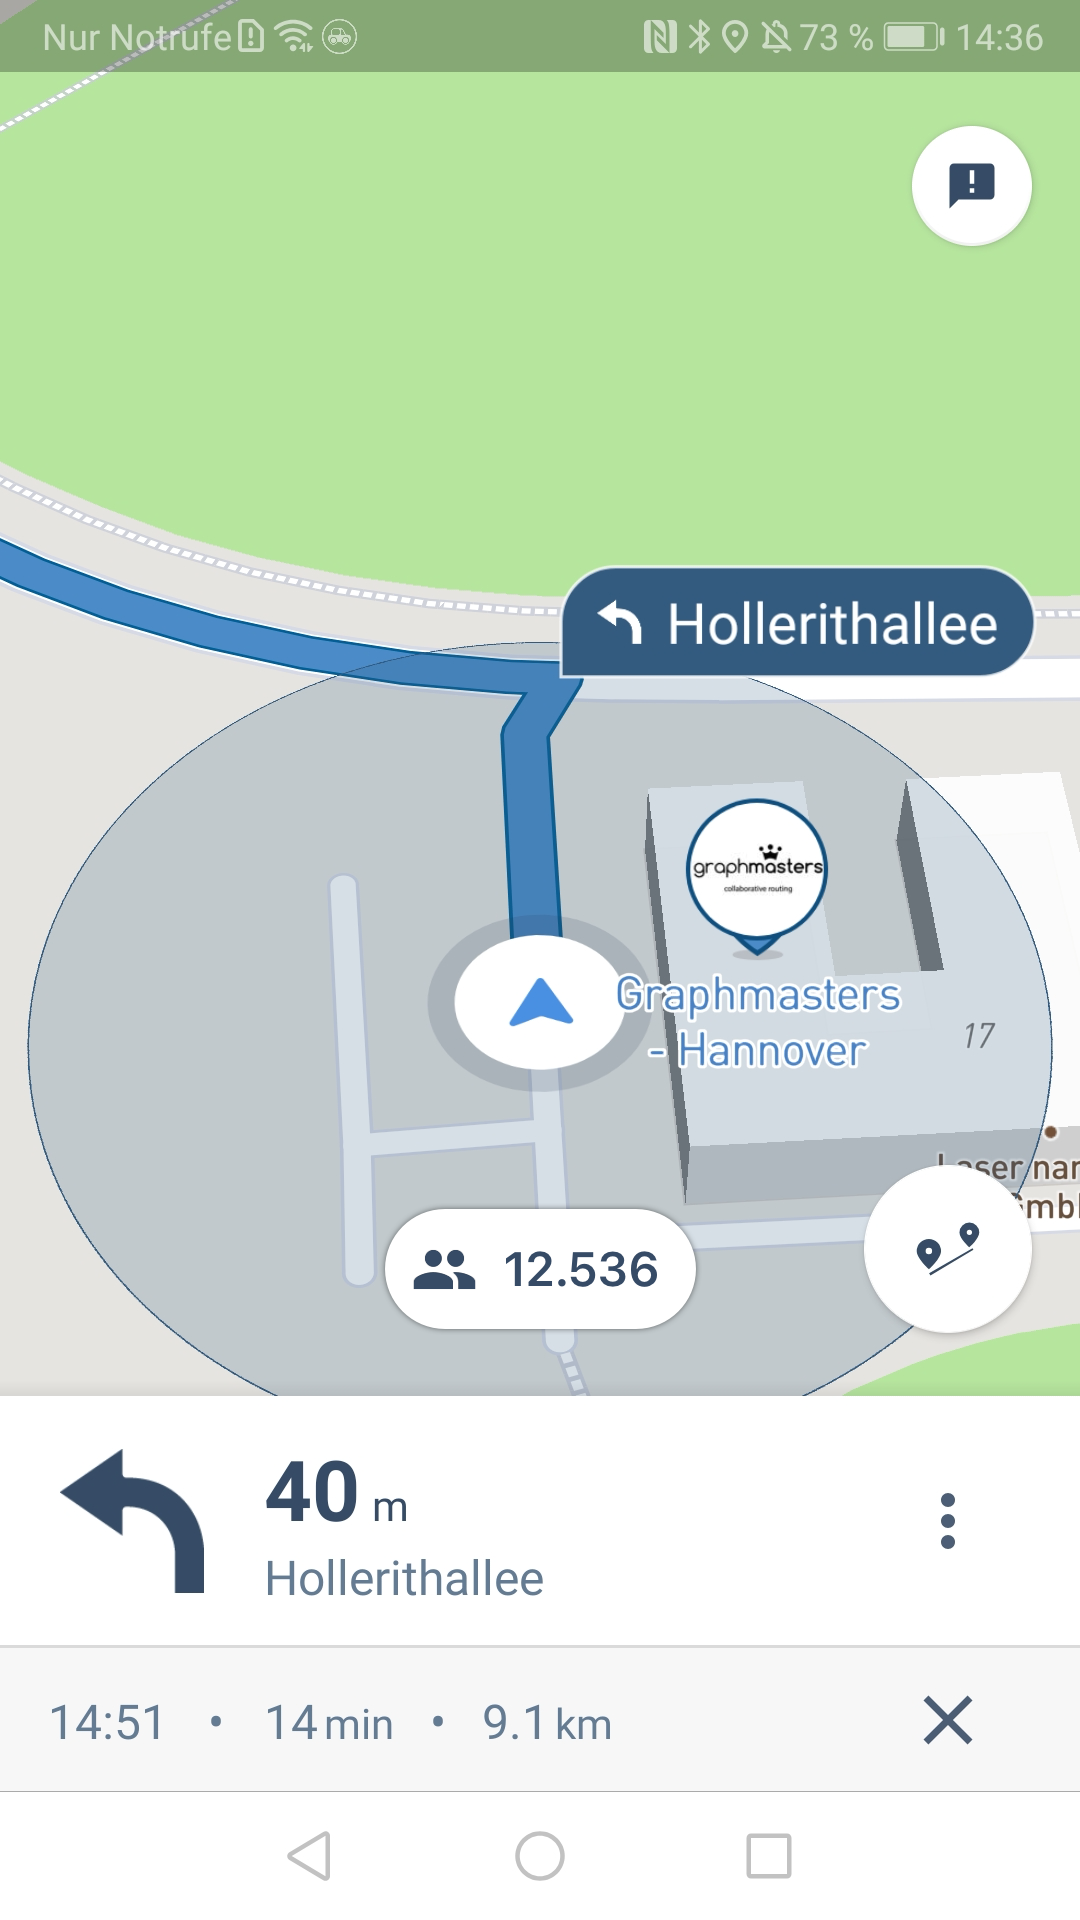
\includegraphics[width=.27\linewidth]{contents/06_model_evaluation/01_integration/res/01_collaborative_routing/prototype_1.png}
    }
    \hspace{.055\linewidth}
    \subfloat[Finales Design der \textit{Affordance} zusammen mit der Anzahl der \textit{End User} in der Umgebung]
    {
        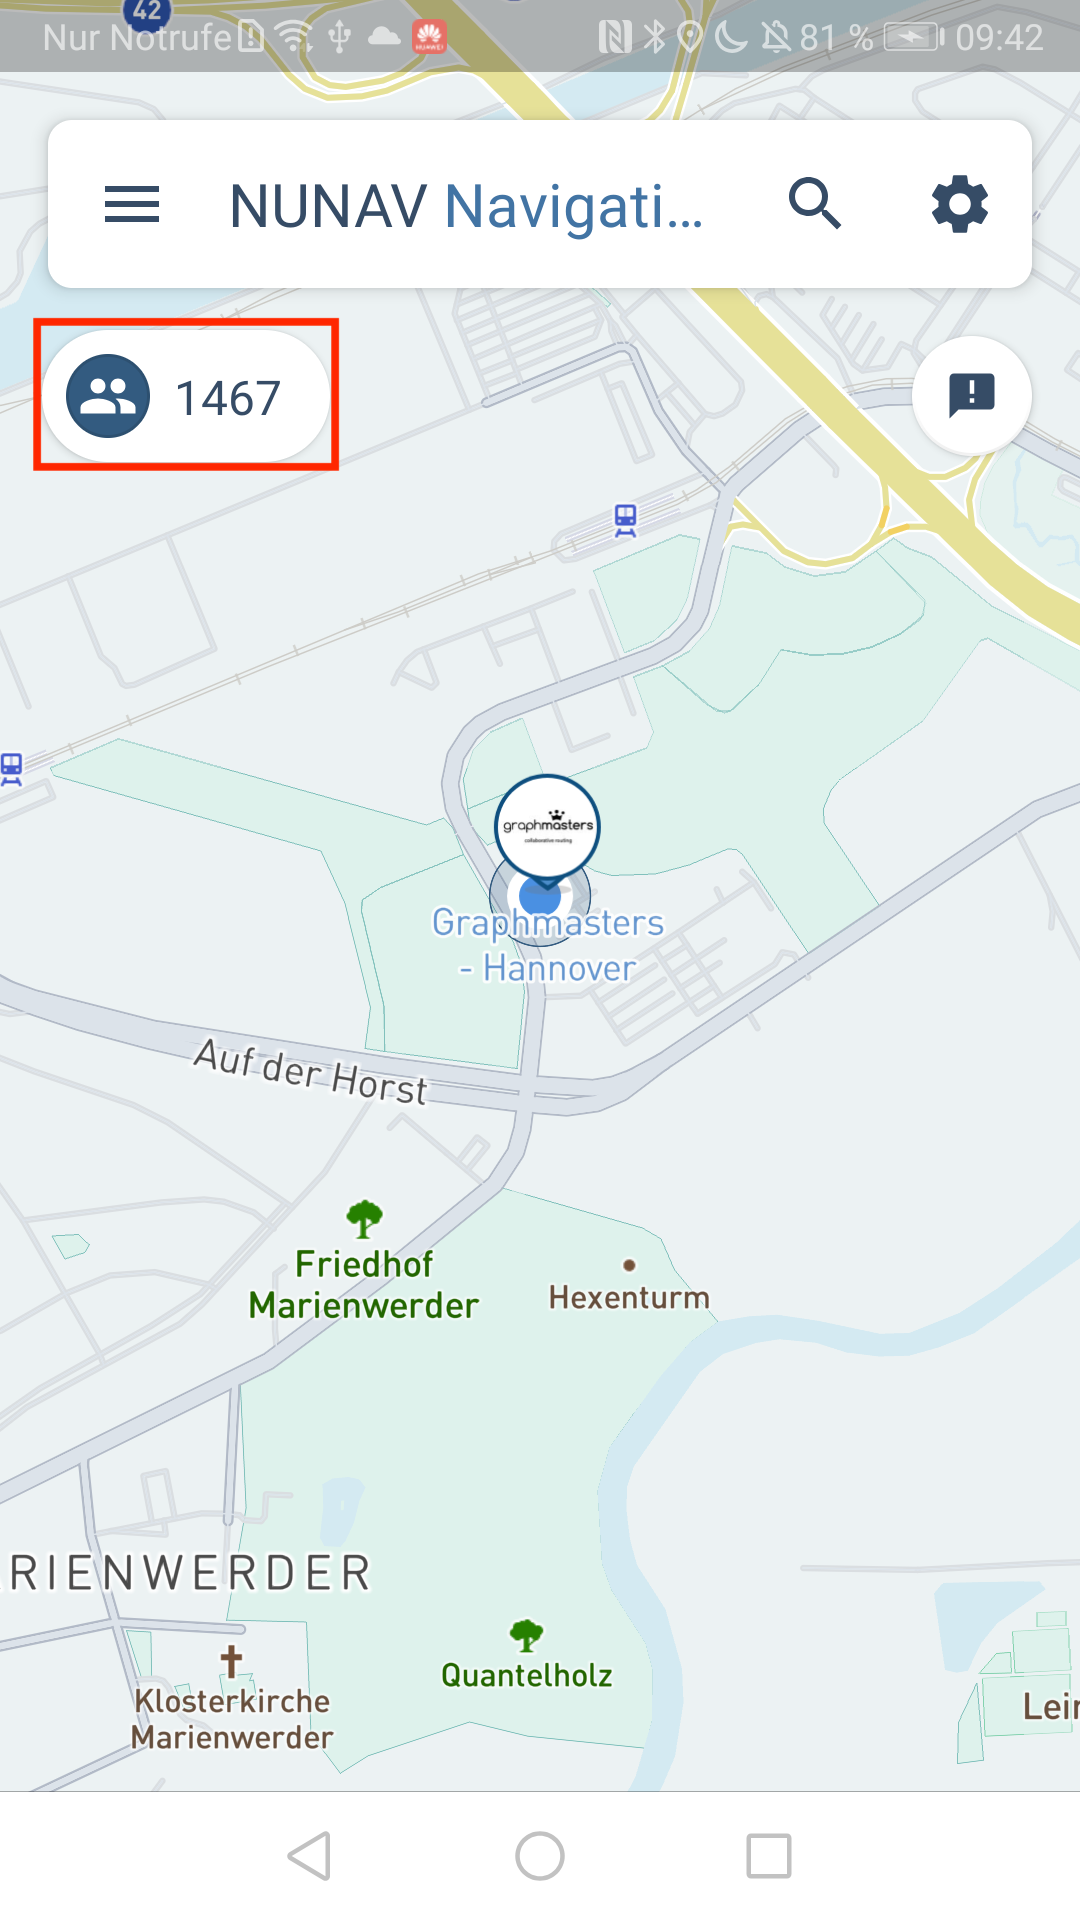
\includegraphics[width=.27\linewidth]{contents/06_model_evaluation/01_integration/res/01_collaborative_routing/final_1.png}
    }
    \hspace{.055\linewidth}
    \subfloat[Finales Design der kurzen Erklärung]
    {
        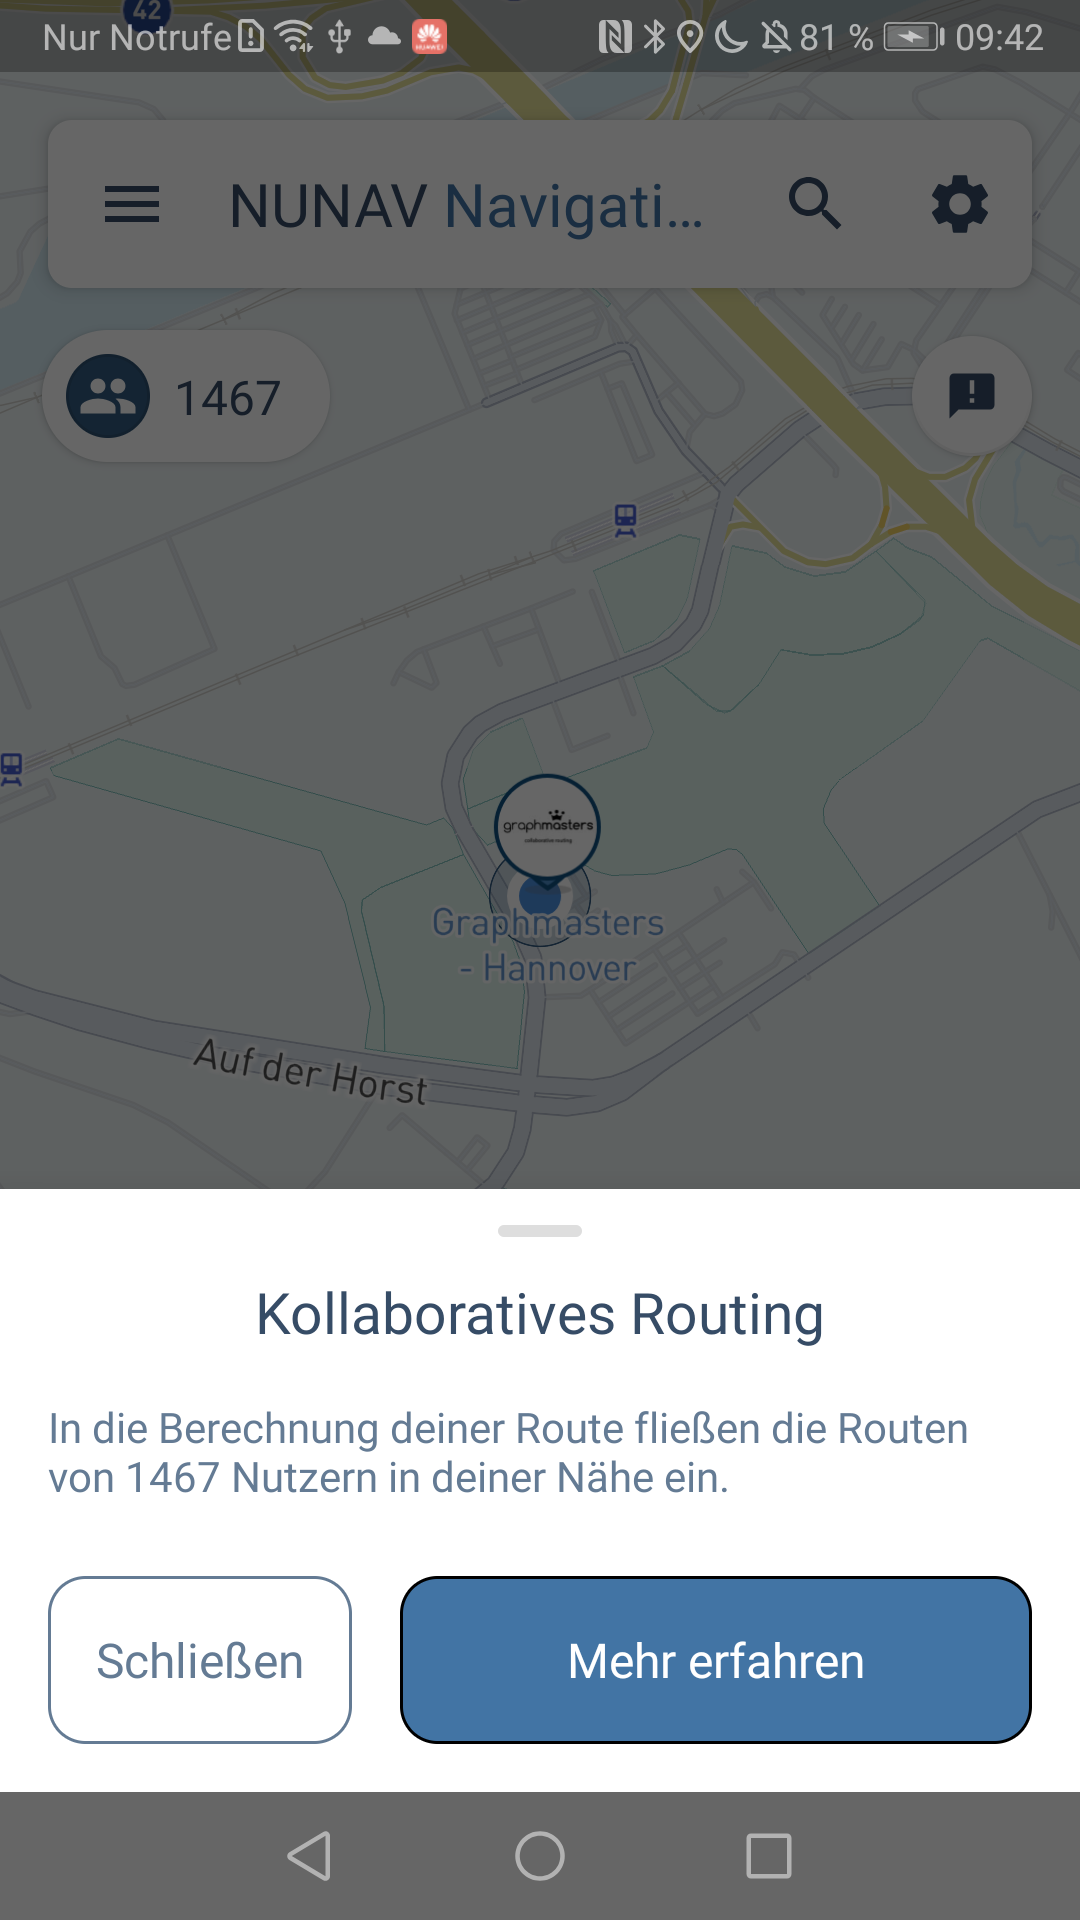
\includegraphics[width=.27\linewidth]{contents/06_model_evaluation/01_integration/res/01_collaborative_routing/final_2.png}
    }
    \caption{Prototyp und finale Designs für die Erklärung zum kollaborativem Routing}
    \label{fig:prototype_collaborative_routing}
\end{figure}